\documentclass[11pt,a4paper]{article}

% Draft: venue-neutral. Switch to acmart/llncs later; keep the body class-agnostic.
\usepackage[T1]{fontenc}
\usepackage[utf8]{inputenc}
\usepackage{amsmath,amssymb,amsthm}
\usepackage{mathtools}
\usepackage{xcolor}
\usepackage[colorlinks=true,linkcolor=blue!50!black,citecolor=blue!50!black,urlcolor=blue!50!black]{hyperref}
\usepackage{microtype}
\usepackage{fullpage}
\usepackage{setspace}
\onehalfspacing
\emergencystretch=1.5em
\usepackage{enumitem}
\usepackage{tikz}
\usetikzlibrary{positioning,fit,arrows.meta,quotes}
\setlist{itemsep=2pt,topsep=4pt}

\newtheorem{definition}{Definition}[section]
\newtheorem{proposition}{Proposition}[section]
\newtheorem{theorem}{Theorem}[section]
\newtheorem{conjecture}{Conjecture}[section]
\newtheorem{example}{Example}[section]
\theoremstyle{remark}
\newtheorem{remark}{Remark}[section]

% ---- notation macros ----
\newcommand{\Ax}{\mathcal{A}}                    % axis set
\newcommand{\Cells}{\mathit{Cells}}
\newcommand{\Dom}{\mathit{dom}}
\newcommand{\open}{\mathsf{open}}
\newcommand{\fixed}{\mathsf{fixed}}
\newcommand{\absent}{\mathsf{absent}}
\newcommand{\vbind}{\mathsf{bind}}
\newcommand{\vscrub}{\mathsf{scrub}}
\newcommand{\vdrill}{\mathsf{drill}}
\newcommand{\vpivot}{\mathsf{pivot}}
\newcommand{\vrelayout}{\mathsf{relayout}}
\newcommand{\vact}{\mathsf{act}}
\newcommand{\vback}{\mathsf{back}}
\newcommand{\TT}{\mathcal{T}}                    % view-type catalogue
\newcommand{\QQ}{\mathcal{Q}}
\newcommand{\LL}{\mathcal{L}}
\newcommand{\Sig}{\Sigma}
\newcommand{\addr}{\mathit{addr}}
\newcommand{\src}{\mathit{source}}
\newcommand{\acts}{\mathit{acts}}
\newcommand{\coord}{\mathit{coord}}
\newcommand{\grain}{\mathit{grain}}
\newcommand{\pop}{\mathit{pop}}
\newcommand{\rank}{\mathit{rank}}

\title{One Open Axis: Vector Views and a Navigation State Machine\\
for Decentralised Observation Cubes}
\author{Draft --- author list TBD}
\date{2026-07-12 (working draft)}

\begin{document}
\maketitle

\begin{abstract}
We propose \emph{vector views}, a deliberately weakened view algebra over
observation cubes in which every screen fixes all but at most one axis, and all
analytical power comes from \emph{chaining} such views. We formalise the user
interface as a pushdown state machine whose states are view frames---axis roles
($\open$/$\fixed$) plus a presentation \emph{layout}---and whose alphabet is six
interaction verbs ($\vbind$, $\vscrub$, $\vdrill$, $\vpivot$, $\vrelayout$,
$\vact$). Each state is grounded in a typed command--query interface to the data
layer, so the formal description and the running application cannot drift. We
prove the machine preserves the one-open-axis invariant, show its states are
URL-addressable, and characterise its expressiveness relative to the cube
algebra. We instantiate the model in Granergize, a Solid-based application for
building-energy data, where the formalisation exposed undeclared data accesses
and made a latent design decision explicit.
\end{abstract}

\section{Introduction}\label{sec:intro}

Personal data stores such as Solid pods~\cite{solid} promise user-controlled data
that applications visit rather than own. For quantitative domains---in our case,
energy consumption of commercial buildings---the data forms a natural
multidimensional space: every number is an observation positioned on a small set of
dimensions (which building or region, which measured quantity, which period, visible
to whom). The analytical literature offers a mature formalism for such spaces, the
data cube with its OLAP operations (slice, dice, roll-up, drill-down,
pivot)~\cite{gray1997,codd1993}, and mature vocabularies for publishing them (the RDF
Data Cube~\cite{qb} alongside SOSA/SSN~\cite{sosa} for raw observations).

For the \emph{user interface} of such an application, however, the cube algebra is
the wrong target, for two reasons:

\begin{itemize}
\item \textbf{Too powerful for the audience.} The intended users (building
  operators, not analysts) ask concrete questions---\emph{how did my hall's
  electricity develop?}, \emph{who can see this building?}, \emph{how does my
  district compare?}---each of which varies a single aspect while holding the rest
  constant. Interfaces that expose free axis composition (pivot tables, cube
  browsers) demand that users \emph{construct} a query; our users \emph{recognise}
  answers.
\item \textbf{Too powerful for the substrate.} A federation of pods has no global
  corpus: the reachable data is assembled at read time from the user's own store,
  grants received from peers, and spatially gated public registers. Arbitrary cube
  operations presuppose an indexed whole; a decentralised application can honestly
  offer only \emph{views over what is reachable}.
\end{itemize}

At the same time, describing the UI \emph{informally}---prose specifications,
hand-drawn flow diagrams---loses precisely what the cube model provides: a checkable
correspondence between what a screen shows and which data it draws on. Between the
full cube algebra and free-form prose we found a gap: a formalism strong enough to
describe every screen and interaction, weak enough to be intuitive, and mechanically
tied to the data-access layer. This paper fills that gap with three contributions:

\begin{enumerate}
\item \textbf{Vector views} (\S\ref{sec:frames}): a view is a \emph{frame} over the
  observation cube---every axis assigned a role, with \emph{at most one axis
  open}---plus a \emph{layout} admissible for that frame. The one-open-axis
  rule (``a vector, not a matrix'') is the deliberate power cut below OLAP.
\item \textbf{Navigation as a state machine} (\S\ref{sec:machine}): the UI is a
  pushdown machine whose states are (frame, valuation, layout) triples --- atomic
  screens, or statechart-style AND-compositions of vectors for detail screens ---
  and whose alphabet is six verbs. Analytical power is recovered by \emph{chaining}: every
  navigation step closes one axis and opens another. We show the machine preserves
  the vector rule, that its navigational component is URL-addressable, and
  characterise its expressive reach relative to the cube algebra.
\item \textbf{Grounding in a typed command--query interface} (\S\ref{sec:grounding}):
  every state declares the read operations that populate it and the write operations
  its $\vact$ transitions dispatch, against an application-wide intent catalogue with
  RDF-typed parameters. The state machine is thus not documentation \emph{about} the
  application but a specification the application can be checked against.
\end{enumerate}

We instantiate the model in Granergize (\S\ref{sec:instantiation}), a React/Solid
application for building-energy data, and discuss what the formalisation caught
(\S\ref{sec:caught}).

\section{A running example}\label{sec:running}

Alice operates three logistics halls around Nuremberg. Her pod holds each hall's
master data and yearly meter readings; a peer, GEG Logistik, has granted her two
of theirs; a public statistics register covers her district. One number in this
space---say, \emph{the Feucht hall's electricity consumption in 2023, as visible
to Alice}---is a point on four coordinates: \emph{which building} (space),
\emph{which quantity} (metric), \emph{which year} (time), \emph{visible to whom}
(agent).

Alice's session in the redesigned application:

\begin{enumerate}
\item She opens the \textsf{Buildings} tab: a map of the five reachable halls.
  One coordinate varies across the marks---the building; everything else is
  either irrelevant here (metric, time) or pinned (the viewer is Alice). She
  narrows to her own halls with a \emph{source} filter and switches the same set
  to a list; the membership does not change, only the layout.
\item She clicks the Feucht hall. The varying coordinate is now \emph{fixed}: one
  building, its detail page. The page offers her the next questions, one
  coordinate each: the hall's metric mix (electricity, heat, water as plain
  figures---now the \emph{metric} varies), each metric's development (a line
  chart---the \emph{year} varies), and who can see the hall (an access
  list---the \emph{agent} varies).
\item She follows electricity into its trend, scrubs the year slider, and goes
  back; then she opens the access list and shares the hall with her consultant
  ---a write action offered in place, on the entity the page has fixed.
\item The address bar has tracked every step
  (\texttt{/building?ref=\ldots\&m=electricity}); she pastes the trend's URL to a
  colleague, who lands on the same view---minus Alice's private browsing trail.
\end{enumerate}

At no point does the interface show two varying coordinates at once: no
buildings\,$\times$\,years matrix, no pivot table. Every screen answers one
question of the form ``vary \emph{this}, hold the rest''; moving between
questions is a click that pins the varying coordinate and releases another. The
rest of the paper makes this precise: the coordinates are the axes of an
observation cube (\S\ref{sec:prelim}), each screen is a \emph{vector view}
(\S\ref{sec:frames}), Alice's session is a run of a state machine over six verbs
(\S\ref{sec:machine}; Example~\ref{ex:chain} replays steps 1--3 formally), and
every screen's content and actions are declared against the data layer's
command--query interface (\S\ref{sec:grounding}).

\section{Preliminaries: the observation cube over pods}\label{sec:prelim}

\subsection{Cells and the cube}

\begin{definition}[Observation cube]\label{def:cube}
Fix the axis set
\[
\Ax = \{\mathit{space},\ \mathit{metric},\ \mathit{time},\ \mathit{agent}\}
\]
with value domains $\Dom(a)$ for $a \in \Ax$:
$\Dom(\mathit{space})$ the features of interest (building IRIs and region IRIs in an
administrative containment hierarchy, municipality $\subset$ district $\subset$
state); $\Dom(\mathit{metric})$ the observed-property IRIs; $\Dom(\mathit{time})$
periods (years, or timestamps for sub-hourly series; resolution is a depth on this
axis); $\Dom(\mathit{agent})$ WebIDs. A \emph{cell} is a tuple
\[
c = \bigl(\,\phi \in \prod_{a\in\Ax}\Dom(a),\; \mu,\; \alpha\,\bigr)
\]
of a coordinate $\phi$, a measure $\mu$, and interpretive attributes $\alpha$ (unit;
aggregation function $\varnothing/\Sigma$ and sample size $n$ for rolled-up cells;
reference area for normalised readings). A \emph{data space} $D$ is a set of cells;
we write $\Cells(D)$ for it and $\phi_a(c)$ for the coordinate of $c$ on axis $a$.
\end{definition}

The agent axis is unusual: access is modelled as a first-class coordinate
($c$ is in the cube \emph{as seen by} $\phi_{\mathit{agent}}(c)$) rather than an
out-of-band permission system; \S\ref{sec:agentaxis} motivates this.

Two RDF serialisations carry cells, deliberately unaligned at the triple level and
converged only in the application's typed object layer: raw first-party measurements
are \texttt{sosa:Observation}s (the coordinates are properties on the fact:
\texttt{hasFeatureOfInterest}, \texttt{observedProperty}, \texttt{resultTime},
\texttt{hasResult}), while aggregates and official statistics are
\texttt{qb:Observation}s in \texttt{qb:DataSet}s whose dimensions mirror the same
axes~\cite{qb,qb4st}. A QB cell is a roll-up of SOSA cells; both levels share the
same IRIs as keys (building IRI, region-code IRI, metric IRI, WebID,
\texttt{xsd:gYear}), which keeps raw data, aggregates, and file-based import/export
joinable.

\subsection{Partiality}\label{sec:partiality}

The cube is \emph{virtual and partial}. There is no registry of buildings and no
corpus of observations; the reachable cell set is assembled at read time from three
provenance tiers---\emph{owned} (the user's pod), \emph{granted} (folded from
append-only sharing logs), and \emph{open} (public registers, queryable only through
spatial gates such as a bounding box or region code). Formally, the application
never evaluates a view against $D$ but against a reachable subspace
$D_{u,\pi} \subseteq D$ indexed by user $u$ and discovery context $\pi$ (the gates
issued so far), with $D_{u,\pi}$ monotone in the \emph{discovery} context $\pi$
at fixed grant state --- discovery only ever adds, whereas visibility is
grant-relative: a revocation (\texttt{RevokeBuildingAccess},
Appendix~\ref{app:writes}) shrinks $D_{u,\pi}$ by changing $u$'s grants, not
$\pi$. Consequently no view may claim
exhaustiveness: absence means ``none reachable'', counts are monotone under
discovery, and every displayed figure must state its tier. The formalism below
treats this as a constraint on view semantics, not a footnote.

\section{Vector views}\label{sec:frames}

\subsection{Frames}

\begin{definition}[Frame; vector rule]\label{def:frame}
A \emph{frame} is a function $F : \Ax \to \{\open, \fixed, \absent\}$. Write
$\open(F) = \{a : F(a) = \open\}$ and likewise $\fixed(F)$. $F$ satisfies the
\emph{vector rule} iff $|\open(F)| \le 1$. A frame with $|\open(F)| = 1$ is a
\emph{vector frame}; with $|\open(F)| = 0$ a \emph{cell frame}.
\end{definition}

\begin{definition}[Valuation; view; semantics]\label{def:view}
A \emph{valuation} of $F$ is a function $v$ with domain $\fixed(F)$ and
$v(a) \in \Dom(a)$. Given a reachable subspace $D_{u,\pi}$ and a facet predicate
$\theta$ (below), the \emph{extent} of the view $(F, v, \theta)$ is
\[
[\![\, F, v, \theta \,]\!] \;=\;
\{\, c \in \Cells(D_{u,\pi}) \;:\; \theta(c) \wedge \forall a \in \fixed(F).\
\phi_a(c) = v(a) \,\}.
\]
For a vector frame the extent varies along the single open axis; its projection to
$\Dom(\open(F))$ indexes the \emph{marks} of the display. For a cell frame the
extent is (at most) a single cell.
\end{definition}

Values of fixed axes are chosen by the user through visible controls, and---
crucially---the navigational part of $v$ is encoded in the application URL: a fixed
coordinate \emph{is} a query parameter (\texttt{m=electricity}, \texttt{y=2023},
\texttt{ref=\ldots}). This gives every state a stable, shareable address
(\S\ref{sec:addr}).

\begin{definition}[Facets]\label{def:facets}
A \emph{facet} is a predicate $\theta$ over cells (or over the entities of the open
axis) drawn from a per-type facet vocabulary: the provenance tier
(owned/granted/open), a role filter, a keyword search. Syntactically $\theta$ is a
finite conjunction of atomic comparisons
$\bigwedge_i (\mathit{field}_i \,\mathit{op}_i\, \mathit{value}_i)$ over the
entity's projected schema, with $\mathit{op}$ drawn from a fixed comparator set
per field type (equality and order for numbers, containment for text, presence
tests). Facets constrain the extent; they never change $F$.
\end{definition}

Distinguishing facets from axes is what keeps $\Ax$ at four; earlier designs that
promoted the tier to an axis produced spurious ``views'' differing only in
filtering.

\subsection{Layouts}\label{sec:layouts}

A frame does not determine a unique rendering but a \emph{menu} of admissible
layouts, given by the open axis and the grain of its values:

\begin{center}
\begin{tabular}{lll}
$\open(F)$ & grain / cardinality & admissible layouts \\
\hline
$\varnothing$            & ---            & labelled figure; field list (instance profile) \\
$\{\mathit{space}\}$     & point          & marker map; list \\
$\{\mathit{space}\}$     & region         & choropleth; catalog list; per-region bars \\
$\{\mathit{time}\}$      & series         & line chart / timeline \\
$\{\mathit{metric}\}$    & few values     & \emph{plain numbers} (stat tiles), not a chart \\
$\{\mathit{agent}\}$     & ---            & access/grant list \\
\end{tabular}
\end{center}

Two laws make a layout a view of one collection rather than a collection of its own:
\emph{membership invariance} (all layouts of a frame show the same extent; switching
layout never filters) and \emph{capability invariance} (search, paging and facets
attach to the frame, hence work identically in every layout). The metric-open row
encodes a data-ink judgement into the formalism: a vector of three or four values
does not earn a chart.

\subsection{The agent axis}\label{sec:agentaxis}

Treating access as the fourth axis dissolves a whole application area. ``Who can
see this building?'' is the agent-open vector of a fixed building; ``which
buildings does this person see?'' is the space-open vector of a fixed agent.
Sharing and revocation are then not a separate \emph{Sharing} module but the
mutations available on those two vectors---the same navigation reaches them, and
the bidirectionality (building${}\leftrightarrow{}$agent) is the symmetry of
opening either axis of the pair. In the store the axis is realised by append-only
grant logs whose fold yields cell visibility; the UI needs no vocabulary beyond the
cube's.

\subsection{Why exactly one open axis}\label{sec:whyone}

The rule is a hypothesis about legibility, borne out in design iterations: one open
axis $=$ one human question in one familiar form. Every additional open axis
multiplies the reading instructions a user must reconstruct (``rows are buildings
\emph{and} columns are years \emph{and} colour is the value''). The cube algebra's
answer to a two-axis question---a matrix---is replaced by a \emph{path}: fix a
building, open time; go back; fix the next building. Where a genuine cross-entity
temporal comparison is needed, the model offers it one level up: an \emph{aggregate
entity} (portfolio, operator group, region) is itself a feature whose time-open
vector is a single line. \S\ref{sec:decision} discusses the cost of this
restriction and the one place our implementation historically violated it.

\section{Navigation as a state machine}\label{sec:machine}

Table~\ref{tab:notation} collects the paper's vocabulary --- the cube terms of
\S\ref{sec:prelim}--\S\ref{sec:frames} and the machine terms this section
introduces --- for reference while reading.

\begin{table}[t]
\centering
\small
\begin{tabular}{@{}l@{\quad}p{8.0cm}@{\quad}l@{}}
term (symbol) & one-line meaning & defined \\
\hline
axis ($a \in \Ax$) & a coordinate dimension of the cube (space, metric, time, agent) & Def.~\ref{def:cube} \\
cell ($c$) & one measure at one coordinate, with interpretive attributes & Def.~\ref{def:cube} \\
reachable subspace ($D_{u,\pi}$) & the cells visible to viewer $u$ under discovery context $\pi$ & \S\ref{sec:partiality} \\
frame ($F$) & a role per axis: $\open$, $\fixed$, or $\absent$; at most one $\open$ & Def.~\ref{def:frame} \\
valuation ($v$) & a value for each fixed axis (partly URL-encoded) & Def.~\ref{def:view} \\
facet ($\theta$) & a filter predicate over the extent; never changes $F$ & Def.~\ref{def:facets} \\
extent ($[\![ F, v, \theta ]\!]$) & the cells a view presents & Def.~\ref{def:view} \\
mark ($m$) & one displayed element of the extent, indexed by the open axis & Def.~\ref{def:view} \\
grain & the resolution of an axis's values (building vs region; year vs hour) & \S\ref{sec:layouts} \\
layout ($\ell \in \LL$) & an admissible rendering of a frame (map, list, line, tiles) & \S\ref{sec:layouts} \\
view type ($\tau \in \TT$) & a catalogued screen kind: route, frame(s), layouts, edges & Def.~\ref{def:catalogue} \\
region ($\rho \in R_\tau$) & one vector of an AND-composite screen & Def.~\ref{def:catalogue} \\
state ($q = (\tau, v, \vec{\ell}\,)$) & a concrete screen: type, valuation, layout per region & Def.~\ref{def:machine} \\
configuration ($(q, \gamma)$) & a state plus the trail stack $\gamma$ & Def.~\ref{def:machine} \\
verbs ($\Sig$) & $\vbind$, $\vscrub$, $\vdrill$, $\vpivot$, $\vrelayout$, $\vact$, $\vback$ & Def.~\ref{def:verbs} \\
\end{tabular}
\caption{Notation summary. Cube terms (top) carry the data; machine terms
(bottom) carry the navigation.}
\label{tab:notation}
\end{table}

\subsection{View types and states}

\begin{definition}[View-type catalogue]\label{def:catalogue}
A \emph{view-type catalogue} is a finite set $\TT$ where each type $\tau \in \TT$
declares: a route $r_\tau$; a facet vocabulary $\Theta_\tau$; a source set
$\src(\tau)$ and act set $\acts(\tau)$ (\S\ref{sec:grounding}); a drill target
$\vdrill_\tau \in \TT \cup \{\bot\}$; pivot edges $E_\tau \subseteq \TT$; and a
body that is either
\begin{itemize}
\item \emph{atomic}: one frame $F_\tau$ satisfying the vector rule, with layout
  menu $\LL_\tau \neq \varnothing$; or
\item \emph{composite} (AND-composition): a set $\fixed(\tau) \subseteq \Ax$ of
  shared fixed axes and a finite family of \emph{regions}
  $R_\tau = \{\rho_1, \ldots, \rho_k\}$, each an atomic frame $F_\rho$ with
  $\fixed(F_\rho) \supseteq \fixed(\tau)$ and $|\open(F_\rho)| \le 1$, with its
  own layout menu $\LL_\rho$. The regions render \emph{juxtaposed} and share one
  valuation of $\fixed(\tau)$.
\end{itemize}
An atomic type is the single-region case; we write $R_\tau$ uniformly.
Well-formedness of the edges: a drill target must be reachable by closing the
open axis --- $\fixed(\tau') \subseteq \fixed(\tau) \cup \{\open(F_\rho)\}$
for $\tau' = \vdrill_\tau$ and the originating region $\rho$ --- and a pivot
target must not require coordinates its source lacks,
$\fixed(\tau'') \subseteq \fixed(\tau)$ for $\tau'' \in E_\tau$; both
conditions are checkable over the catalogue.
\end{definition}

\begin{remark}[Juxtaposition, not composition]\label{rem:juxta}
A composite screen shows several vectors \emph{side by side} --- statechart-style
parallel (AND) regions~\cite{harel} over one fixed entity --- but never a
product: no single region encodes two axes jointly, so a rank-$2$ display (a
buildings\,$\times$\,years matrix, say) remains unreachable. Detail pages are
the motivating case (\S\ref{sec:instantiation}): master-data cells, the metric
mix, and the access list are AND-regions sharing the fixed building.
\end{remark}

\begin{definition}[Navigation machine]\label{def:machine}
The \emph{navigation machine} over $\TT$ is the pushdown system
$M = (\QQ, \Sig, \delta, Q_0)$ where
\begin{itemize}
\item states $q = (\tau, v, \vec{\ell}\,) \in \QQ$ with $\tau \in \TT$, $v$ a
  valuation of $\tau$'s fixed axes, and $\vec{\ell} = (\ell_\rho)_{\rho \in R_\tau}$
  a layout per region, $\ell_\rho \in \LL_\rho$; a \emph{configuration} is
  $(q, \gamma)$ with trail stack $\gamma \in \QQ^{*}$;
\item $\Sig = \{\vbind, \vscrub, \vdrill, \vpivot, \vrelayout, \vact, \vback\}$
  (with parameters);
\item $Q_0 \subseteq \QQ$ the tab-entry states (empty stack);
\item $\delta$ as in Definition~\ref{def:verbs}.
\end{itemize}
\end{definition}

The state space is infinite only through $v$ (entity IRIs, years); its quotient by
valuations---the \emph{frame graph} $(\TT, \vdrill_\bullet \cup E_\bullet)$---is
finite and is what designers reason about
(Figure~\ref{fig:framegraph} shows the instantiated one).

\subsection{The verb alphabet}

\begin{definition}[Transitions]\label{def:verbs}
For a configuration $((\tau, v, \vec{\ell}\,), \gamma)$; we write $\ell$ for
$\vec{\ell}$ where regions play no role, and a verb that names an axis or a mark
implicitly names the region $\rho \in R_\tau$ it originates in:
\begin{description}
\item[$\vbind(a, x)$] for $a \in \fixed(F_\tau)$, $x \in \Dom(a)$:
  \[ ((\tau, v, \ell), \gamma) \;\to\; ((\tau, v[a \mapsto x], \ell), \gamma). \]
\item[$\vscrub(a)$] the timed iteration of $\vbind(a, \cdot)$ over the order of
  $\Dom(a)$ (sugar: $\vscrub = \vbind^{*}$).
\item[$\vdrill(m)$] for $a = \open(F_\rho)$, $\tau' = \vdrill_\tau \neq \bot$, and
  $m$ a mark of the extent (carrying its open-axis coordinate $\coord(m)$):
  \[ ((\tau, v, \ell), \gamma) \;\to\;
     \bigl(\bigl(\tau',\; (v \cup \{a \mapsto \coord(m)\})\!\restriction_{\fixed(F_{\tau'})},\; \ell'_0\bigr),\;
     \gamma \cdot (\tau, v, \ell)\bigr). \]
\item[$\vpivot(\tau'')$] for $\tau'' \in E_\tau$:
  \[ ((\tau, v, \ell), \gamma) \;\to\;
     \bigl(\bigl(\tau'',\; v\!\restriction_{\fixed(F_{\tau''})},\; \ell''_0\bigr),\;
     \gamma \cdot (\tau, v, \ell)\bigr). \]
\item[$\vrelayout(\rho, \ell')$] for $\ell' \in \LL_\rho$:
  \[ ((\tau, v, \vec{\ell}\,), \gamma) \;\to\; ((\tau, v, \vec{\ell}\,[\rho \mapsto \ell']), \gamma). \]
\item[$\vact(i, p)$] state unchanged; dispatch write intent $i(p)$ with
  $p \subseteq v$; invalidate the states whose $\src$ depends on $i$'s effect.
\item[$\vback$]
  $((\tau, v, \ell), \gamma \cdot q') \to (q', \gamma)$; on the empty stack, fall to
  the type's declared collection fallback.
\end{description}
Here $\ell'_0, \ell''_0$ are the targets' default layouts.
\end{definition}

$\vdrill$ is the \emph{close} half of chaining: the open axis of $\tau$ becomes a
fixed coordinate of $\tau'$, whose own frame opens a successor axis (or none,
landing on a cell view). $\vpivot$ is the \emph{open} half: from an entity-fixed
state, open a different axis on the same entity (a building's metric mix opens
\emph{metric}; its trend opens \emph{time}; its access section opens \emph{agent};
an agent's building list opens \emph{space}), or cross to a related entity along a
single-valued edge (building $\to$ operator). Because pivots fan out, the trail is
a genuine stack, not a linear history: $M$ is a pushdown system over the finite
frame graph. Deep entry (a shared URL) is the empty-stack case.

\begin{example}[A chain]\label{ex:chain}
Alice's session from \S\ref{sec:running}, steps 1--3:
\emph{``How did the Feucht hall's electricity develop, and who else can see it?''}
\begin{align*}
\underbrace{(\textsf{Buildings}, \{\}, \textsf{map})}_{\text{space open}}
&\xrightarrow{\ \vdrill(b_1)\ }
\underbrace{(\textsf{BuildingDetail}, \{s{=}b_1\}, \cdot)}_{\text{regions: metric open} \,\|\, \text{agent open}} \\
&\xrightarrow{\ \vpivot(\textsf{Trend})\ }
\underbrace{(\textsf{Trend}, \{s{=}b_1, m{=}\mathrm{el}\}, \textsf{line})}_{\text{time open}}
\xrightarrow{\ \vback\ }
(\textsf{BuildingDetail}, \{s{=}b_1\}, \cdot)
\end{align*}
Each navigation closes one axis and opens another, and every region along the
run holds at most one open axis. The access question needs no further step: the
composite's agent-open region \emph{is} the access list.
\end{example}

\subsection{Invariant preservation}

\begin{theorem}[Vector invariant]\label{thm:invariant}
If every region of every $\tau \in \TT$ satisfies the vector rule and $\TT$ is
closed under $\vdrill_\bullet$ and $E_\bullet$, then every region of every
reachable configuration of $M$ satisfies the vector rule.
\end{theorem}

\begin{proof}
Induction over runs. States in $Q_0$ are catalogue types, which satisfy the rule by
declaration. $\vbind$, $\vscrub$, $\vrelayout$, $\vact$ do not change the frame.
$\vdrill$ and $\vpivot$ move to catalogue types, all of whose regions satisfy
the rule by assumption; $\vback$ pops to a previously reachable state.
\end{proof}

The proof is trivial \emph{because the catalogue is code} (\S\ref{sec:grounding}):
the content of the theorem is that the closure condition is machine-checkable at
build time---a drill target that opened two axes is rejected when the catalogue is
validated, before any screen exists.

\subsection{Addressability}\label{sec:addr}

\begin{proposition}[URL addressing]\label{prop:addr}
Assume (R) the routes $r_\tau$ are pairwise distinct across $\TT$ and (E)
$\mathit{encode}$ is injective per type. Then
$\addr(\tau, v, \vec{\ell}\,) = r_\tau \cdot
\mathit{encode}(v\!\restriction_{\mathrm{nav}}, [\vec{\ell}\,])$ --- the route plus
the query-parameter encoding of the navigational valuation (and the layouts where
remembering them matters) --- is total and injective on reachable states, modulo
the trail and any layouts omitted from the encoding.
\end{proposition}

\begin{proof}
Totality: every state has a type, and every type a route and encodable valuation.
Injectivity: (R) recovers $\tau$; (E) recovers $v\!\restriction_{\mathrm{nav}}$
and the encoded layouts.
\end{proof}

\emph{Decoding} is deliberately weaker: it is relative to a context
$(\sigma, u)$ of browsing session and viewer. An absent parameter resolves by
precedence URL $>$ $\sigma$-remembered $>$ type default
(Appendix~\ref{app:uri}), and a present coordinate outside the viewer's
reachable domain is clamped. Hence $\mathit{decode}_{\sigma,u} \circ \addr =
\mathrm{id}$ holds exactly for the \emph{fully explicit} address; the canonical,
defaults-omitted address trades the exact round-trip for stable, clean links ---
its decode is context-dependent by design. A shared address, moreover, evaluates
against the \emph{recipient's} reachable subspace $D_{u',\pi'}$: the state is
stable, its extent viewer-relative --- the addressing-level face of partiality
(\S\ref{sec:partiality}).

The trail is likewise excluded from $\addr$: a shared link must not replay the
sender's browsing path, so the stack lives in session history state, not in the
address. Consequences: reload and share are total; the state machine \emph{is}
the specification of the URL scheme; and parameters not derivable from some
type's frame are dead and can be linted away.

\subsection{Expressiveness}\label{sec:express}

Call $S \subseteq \Cells(D_{u,\pi})$ a \emph{rank-$k$ slice} if $S$ is the extent of
a frame with $k$ open axes. A single state of $M$ presents a rank-$\le\!1$ slice;
the OLAP algebra reaches rank-$k$ slices for any $k$ plus arbitrary dicing, so
vector views are strictly weaker \emph{per state}.

\begin{proposition}[Reach of runs]\label{prop:reach}
Along a run, $M$ presents any finite union of rank-$1$ slices: for a rank-$2$
slice over axes $(a,b)$, the run that iterates $\vbind(a, x)$ over
$x \in \pi_a(S)$, at each step presenting the rank-$1$ slice with $a$ fixed at $x$
and $b$ open, enumerates $S$ --- at a cost of $\Theta(|\pi_a(S)|)$ navigations,
the deliberate price of the vector rule for genuinely rank-$2$ questions.
Roll-up is recovered through aggregate entities:
a portfolio, operator group, or region is a feature whose cells are QB roll-ups of
member cells, so a ``cross-entity'' question is a rank-$1$ slice one level up.
\end{proposition}

What is \emph{not} reachable, by design: simultaneous presentation of a rank-$2$
slice, arbitrary computed measures, and ad-hoc dimension hierarchies.

\begin{conjecture}\label{conj:sufficiency}
Rank-$1$ presentation, chaining, and aggregate entities suffice for the
recognition-style competency questions of the target audience
(\S\ref{sec:cq}); rank-$2$ needs remain expressible as a sanctioned extension
(\S\ref{sec:decision}).
\end{conjecture}

\section{Grounding: the typed command--query interface}\label{sec:grounding}

The machine so far describes navigation; its states must also say \emph{where their
content comes from}. The application's data layer exposes a single catalogue of
\emph{intents} obeying command--query separation~\cite{meyer}: \emph{read intents}
return values (\texttt{FindBuildings}, \texttt{GetBuilding},
\texttt{GetObservationYear}, \texttt{WhoHasAccess}, \texttt{SharedWithMe},
\texttt{FindRegionalStatistics}, \texttt{FindNearbyInstallations}, \ldots) and
\emph{write intents} return outcomes (\texttt{ShareBuilding},
\texttt{SaveObservation}, \texttt{CreateAggregation}, \ldots). Every intent's
parameter schema is RDF-typed---each parameter declares node kind (IRI vs literal),
class or datatype range, and cardinality---and a compile-time witness ties the
schema to the implementation, so the catalogue cannot drift from the code. (The
witness checks field-name-set equality against the implementation's parameter
types, not full value typing --- the type system cannot express IRI-hood, so
deeper rigour would not pay.)

The grounding is two total mappings declared per view type:

\begin{description}
\item[$\src(\tau)$] the read intents (with which parameters are supplied by $v$)
  whose results populate $\tau$'s extent. E.g.\ the building-detail type sources
  $\texttt{GetBuilding}\{s\}$, $\texttt{GetObservationYear}\{s, t\}$ per year, and
  $\texttt{WhoHasAccess}\{s\}$.
\item[$\acts(\tau)$] the write intents reachable through $\vact$, computed per
  instance by an affordance resolver (state guards over the object and viewer:
  own vs granted, has-energy, \ldots), so a context menu and a command palette can
  never disagree.
\end{description}

Appendix~\ref{app:intents} lists the full catalogue with each intent's parameter
schema; Appendix~\ref{app:uri} gives the URI scheme realising
Proposition~\ref{prop:addr}.

Two properties follow. \textbf{Auditability}: a screen that reads data not
reachable through $\src(\tau)$ is a specification violation; in our implementation
the audit surfaced several (\S\ref{sec:gaps}). \textbf{Front-door uniformity}:
because states are addressable (Prop.~\ref{prop:addr}) and intents are typed,
non-visual front doors---a command palette, deep links, an LLM translating natural
language to $\{name, params\}$ objects---operate on the \emph{same} machine: a
palette query compiles to a facet/selector over the open axis, a palette command is
an $\vact$, a navigation result is an $\addr$. Words in, cube coordinates out.

\section{Instantiation: Granergize}\label{sec:instantiation}

\subsection{The catalogue}

Granergize's redesign resolves into ten view types, whose frame graph is drawn
in Figure~\ref{fig:framegraph}; the load-bearing ones, with
open axis in bold:

\begin{description}
\item[Buildings] \textbf{space} open at building grain; agent fixed at the viewer
  (tier, role, search as facets); layouts map $\rightleftarrows$ list; drill
  $\to$ building detail.
\item[Building detail] space fixed; an AND-composite
  (Definition~\ref{def:catalogue}) whose parallel regions are the master-data
  cells, the \textbf{metric}-open mix (stat tiles and benchmark bars, the four
  benchmark rows being four QB cells differing only in refArea/roll-up), and the
  \textbf{agent}-open access list. The per-metric trend (\textbf{time} open) is
  a separate state reached by pivot, as are the operator (agent entity) and the
  open-data surroundings.
\item[Observations] one building's numbers: two states chained by pivot,
  metric open (tiles; time fixed and scrubbable) $\rightleftarrows$ time open
  (line; metric fixed).
\item[Aggregations] \textbf{space} open at region grain; the \emph{statistic} is
  the primary entity (each covers the territory; the region is its breakdown), so
  the list layout is a statistics catalog and the map layout a choropleth with
  explicit no-data rendering for partial coverage; drill $\to$ statistic detail,
  an AND-composite whose parallel regions are the headline cells, the
  \textbf{time}-open trend, and the \textbf{space}-open per-district breakdown.
\item[Agents] \textbf{agent} open; drill $\to$ agent detail, whose two space-open
  lists (``can see'', ``shares with me'') realise the axis's bidirectionality.
  This type absorbs what was previously a separate Sharing area.
\item[Rooms] a saved agent $\times$ space \emph{selection} (a reusable sharing
  context): both axes fixed as sets; not a fifth axis.
\end{description}


\begin{figure}[t]
\centering
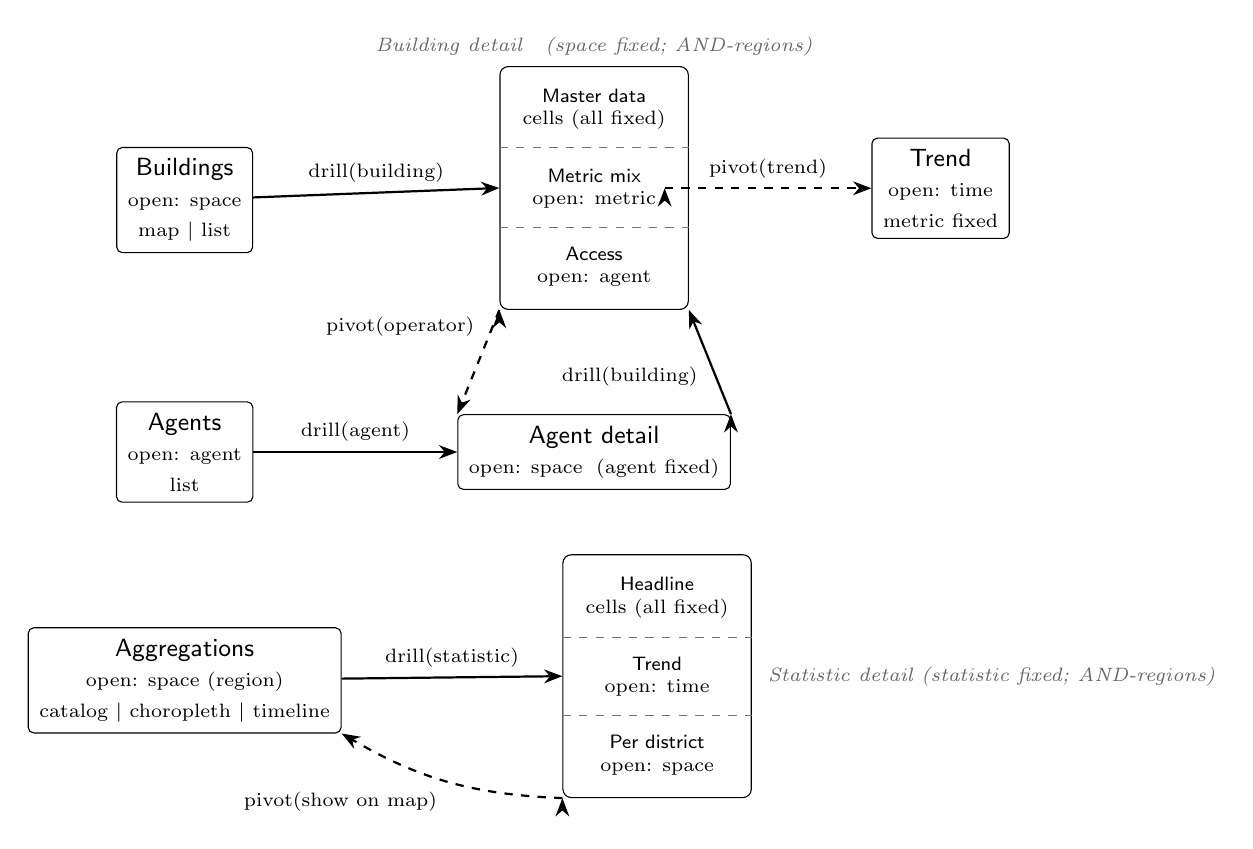
\begin{tikzpicture}[
  st/.style={draw, rounded corners=2pt, align=center, font=\small,
             inner sep=4pt, minimum height=9mm},
  sub/.style={align=center, font=\scriptsize, inner sep=3pt, minimum height=6mm},
  lab/.style={font=\scriptsize\itshape, text=black!60},
  dr/.style={-{Stealth}, thick},
  pv/.style={-{Stealth}, thick, dashed},
  every edge quotes/.style={font=\scriptsize, auto},
  node distance=4mm and 9mm]

% ---- the entity machine -------------------------------------------------
\node[st] (B) at (0,0.2) {\textsf{Buildings}\\ \scriptsize open: space\\ \scriptsize map $|$ list};
\node[sub] (FD) at (5.2,1.35) {\textsf{Master data}\\ cells (all fixed)};
\node[sub] (MM) at (5.2,0.35) {\textsf{Metric mix}\\ open: metric};
\node[sub] (AC) at (5.2,-0.65){\textsf{Access}\\ open: agent};
\node[draw, rounded corners=3pt, fit=(FD)(MM)(AC), inner sep=5pt] (BD) {};
\draw[dashed, black!55] (BD.west |- 0,0.87) -- (BD.east |- 0,0.87);
\draw[dashed, black!55] (BD.west |- 0,-0.15) -- (BD.east |- 0,-0.15);
\node[lab, anchor=south] at (BD.north) {Building detail \; (space fixed; AND-regions)};
\node[st] (TR) at (9.6,0.35) {\textsf{Trend}\\ \scriptsize open: time\\ \scriptsize metric fixed};
\node[st] (AG) at (0,-3.0) {\textsf{Agents}\\ \scriptsize open: agent\\ \scriptsize list};
\node[st] (AD) at (5.2,-3.0) {\textsf{Agent detail}\\ \scriptsize open: space \;(agent fixed)};

\draw[dr] (B) edge["drill(building)"] (BD.west);
\draw[pv] (MM.east) edge["pivot(trend)"] (TR.west);
\draw[pv] (BD.south west) edge["pivot(operator)"'{pos=.35}] (AD.north west);
\draw[dr] (AG) edge["drill(agent)"] (AD);
\draw[dr] (AD.north east) edge["drill(building)"{pos=.55}] (BD.south east);

% ---- the statistics machine ----------------------------------------------
\node[st] (AGGR) at (0,-5.9) {\textsf{Aggregations}\\ \scriptsize open: space (region)\\ \scriptsize catalog $|$ choropleth $|$ timeline};
\node[sub] (HL) at (6.0,-4.85) {\textsf{Headline}\\ cells (all fixed)};
\node[sub] (ST) at (6.0,-5.85) {\textsf{Trend}\\ open: time};
\node[sub] (SD) at (6.0,-6.85) {\textsf{Per district}\\ open: space};
\node[draw, rounded corners=3pt, fit=(HL)(ST)(SD), inner sep=5pt] (SDET) {};
\draw[dashed, black!55] (SDET.west |- 0,-5.35) -- (SDET.east |- 0,-5.35);
\draw[dashed, black!55] (SDET.west |- 0,-6.35) -- (SDET.east |- 0,-6.35);
\node[lab, anchor=west] at (SDET.east) {\;Statistic detail (statistic fixed; AND-regions)};
\draw[dr] (AGGR) edge["drill(statistic)"] (SDET.west);
\draw[pv] (SDET.south west) edge[bend left=14, "pivot(show on map)"{pos=.5}] (AGGR.south east);

\end{tikzpicture}
\caption{The frame graph of Granergize, partitioned into its sub-machines for
legibility: the entity machine (Buildings/Agents, the Building-detail composite,
and the per-metric Trend) and the statistics machine. A box with dashed internal
dividers is an AND-composite (Definition~\ref{def:catalogue}): its regions render
side by side, each holding at most one open axis (Remark~\ref{rem:juxta}). Solid
edges are $\vdrill$ (close the open axis at a mark), dashed edges $\vpivot$ (open
another axis); every edge pushes the trail, and $\vback$ reverses it.
$\vrelayout$ self-loops are omitted---each state lists its layout menu instead.
The tab bar enters a sub-machine at its initial state; the \textsf{Observations}
tab reuses the metric-mix\,$\rightleftarrows$\,trend pair behind a building
picker ($\vbind$), and \textsf{Rooms} (both axes fixed as sets) is omitted.
Every region drawn satisfies the vector rule (Theorem~\ref{thm:invariant}).}
\label{fig:framegraph}
\end{figure}

\subsection{The machine in the running application}

The state machine is not an after-the-fact diagram; its components exist in the
code. Fixed-axis valuations are the URL scheme (pure per-type resolvers own the
encoding); the trail stack is history state pushed at every drill/pivot seam and
popped by the back affordance; layout menus are the per-type view switches; sources
and acts are the intent catalogue with its affordance resolver. What the
formalisation adds is \emph{closure}: one declared catalogue from which the URL
scheme, the navigation graph, and the read/write surface are all derived, with
drift guards in the test suite (the same pattern already proven for the intent
schema itself). An interactive annotated wireframe---each screen rendered beside
its frame, sources, and verb-tagged controls, with the URL bar live---serves as the
shared artefact between design and implementation.

\subsection{Competency questions as reachability}\label{sec:cq}

The project's evaluation harness is organised around competency questions (what a
user wants to find out) and competency tasks (what a user wants to do). Under the
model these acquire exact semantics: a CQ is answered by a \emph{reachable state}
whose vector contains the answer; a CT is a \emph{run} ending in an $\vact$.
``How did my hall's electricity develop?'' is the state $(\textsf{Trend},
\{s{=}h,\, m{=}\mathrm{electricity}\}, \textsf{line})$; ``who can see this
building?'' is $(\textsf{Access}, \{s{=}h\}, \textsf{list})$. Coverage arguments
become path enumeration, and an end-to-end test per CQ/CT is a scripted run of the
machine---which is how the existing browser test suite is already keyed, now with a
formal object to key on. Appendix~\ref{app:cq} works through the project's CQ/CT
catalogue, giving each question its answering state and each task its run.

\section{What the formalisation caught}\label{sec:caught}

\subsection{Undeclared sources}\label{sec:gaps}

Requiring $\src(\tau)$ to be total over catalogued read intents exposed every place
a screen reads data through an ad-hoc path: the aggregation list, the benchmark
rows, the weather overlay, the address book, and the room-membership folds all
reached the store through reactive hooks with no corresponding intent. None was a
bug; all were invisible to every non-UI front door (palette, deep links, LLM,
headless tests). The model turns ``we should probably add read operations for
these'' from a code-review remark into a checkable completeness condition.

\subsection{A real design decision, made visible}\label{sec:decision}

The shipped application contained two views violating the vector rule: a buildings
$\times$ years heatmap and a multi-line chart of all buildings over
time---rank-$2$ slices, useful to power users, overwhelming to the target persona.
The formalism did not decide the question but \emph{stated} it: either adopt
$|\open(F)| \le 1$ and dissolve both into chained vectors (the redesign's
position: per-building trends, plus portfolio-level aggregate entities for the
cross-building question), or sanction $|\open(F)| \le 2$ with the matrix layout as
a marked power view. Because the rule is a declared invariant rather than
folklore, the choice is now a one-line catalogue policy with a test, not a drift.

\subsection{Honest partiality}

Because every state names its sources and every source names its tier, the
partiality discipline of \S\ref{sec:partiality} becomes enforceable per view: an
extent fed by an open-tier source must render its spatial gate (``in this map
view''), never ``all''; a statistic whose refArea dimension covers a subset
renders uncovered regions as explicit no-data. The choropleth's grey is, in this
reading, part of the formalism.

\section{Related work}\label{sec:related}

\paragraph{Cube models.} The data cube operator and OLAP algebra~\cite{gray1997,
codd1993} define the space we restrict; QB4ST~\cite{qb4st} extends the RDF Data
Cube with spatio-temporal dimension semantics matching our space/time axes. Our
contribution is not a cube model but a disciplined weakening of its interface.

\paragraph{Visualization grammars and typologies.} Polaris/Tableau's table
algebra~\cite{polaris} and Vega-Lite's grammar with selections~\cite{vegalite}
couple data queries to encodings declaratively; a vector view is coarser---it
fixes the encoding decision at the frame level (layout menus) precisely to keep the
state space enumerable. Visualization recommendation --- Voyager's
specification-space browsing~\cite{voyager} and Draco's constraint-based design
knowledge~\cite{draco} --- is the natural machinery for \emph{deriving} the
layout menu we currently curate by hand; natural-language interfaces to
visualization (e.g.\ NL4DV~\cite{nl4dv}) parallel our LLM front door one
grammar level down; and the trail of \S\ref{sec:machine} is a navigation-level
cousin of graphical histories for visual analysis~\cite{heer2008}. Brehmer and Munzner's task typology~\cite{brehmer} and
Shneiderman's mantra~\cite{shneiderman} map onto verb sequences: overview $=$ a
collection state, filter $=$ $\vbind$ on facets, details on demand $=$ $\vdrill$.
Bach et al.'s space-time-cube operations~\cite{bach} are, in our terms, frame
transitions: time cutting $=$ time moved to fixed-with-scrub; flattening $=$ time
fixed by aggregation; juxtaposing $=$ iterated $\vbind$. Their descriptive
framework becomes, here, an operational alphabet.

\paragraph{Faceted and set-based browsing.} Faceted browsing~\cite{yee} and
set-pivot browsers such as Parallax~\cite{parallax} popularised filtering and
pivoting over item sets; our facet/axis distinction and the $\vpivot$ verb inherit
from them, with two deltas: the underlying space is a measured cube rather than an
item corpus, and the federation forbids the global counts classic faceted UIs rely
on.

\paragraph{Formal interface models.} Statecharts~\cite{harel} and dialogue models
formalise UI control flow; our machine is a statechart specialised to a domain
(including its AND-decomposition, which we use for detail screens):
states carry cube-theoretic structure (frames), so invariants like the vector rule
and properties like URL-addressability can be stated \emph{about the domain}, not
merely about widgets. The pushdown treatment of navigation history is standard in
program analysis; its application to the back-trail---and the deliberate exclusion
of the stack from the shareable address---appears novel in this setting.

\paragraph{Decentralised applications.} Work on Solid application
architecture~\cite{solid} addresses authentication, access control, and data
discovery; we add a presentation-layer formalism that takes the substrate's
defining property---partiality---as a semantic constraint on views rather than an
implementation nuisance.

\section{Limitations and future work}\label{sec:limits}

The vector rule is a hypothesis about a user population; it warrants an empirical
study (task completion and error rates, vector-chaining vs a matrix baseline, on
the CQ catalogue). The layout menu is currently hand-curated per open-axis/grain
pair; deriving it from mark cardinality and data-ink heuristics is open. The
sufficiency conjecture (Conj.~\ref{conj:sufficiency}) needs a sharper statement of
the question class to be provable. The pushdown framing is so far descriptive
--- no decidability is exploited; model-checking reachability and invariants
over the finite frame graph is the natural next step alongside the empirical
study. $\vscrub$ is modelled as iterated $\vbind$,
which loses its perceptual role (animation as a display of the time axis); a
richer treatment would type it as a temporary opening of a fixed axis. Finally,
the LLM front door currently emits single intents; emitting \emph{runs} (verb
sequences reaching a state that answers a question) is a natural next step, and
the state machine gives the target language for it.

\section{Conclusion}

We described a user interface not as a set of screens but as a pushdown state
machine over frames of an observation cube, with one deliberate
impoverishment---at most one open axis per state---and one deliberate
enrichment---every state grounded in a typed command--query catalogue. The
impoverishment buys legibility for non-technical users and a finite, checkable
frame graph; the enrichment buys non-drifting documentation, uniform front doors,
and honest provenance over a decentralised, partial data space. The cube stays;
the algebra the user touches shrinks to six verbs and one rule: \emph{one open
axis, then chain}.

\bibliographystyle{plain}
\bibliography{paper-vector-navigation}

\appendix

\cleardoublepage
\section{The intent catalogue}\label{app:intents}

The catalogue as implemented (46 intents; the compile-time witness of
\S\ref{sec:grounding} keeps this appendix's schemas equal to the code's). Each
parameter is written $\mathit{name} : \mathit{range}$ with a cardinality suffix:
none $=$ required single (\textsf{one}); \texttt{?} $=$ optional (0--1);
\texttt{+} $=$ required list ($\ge$1); \texttt{*} $=$ optional list (0+). A
parameter whose range is a \emph{class} IRI (\texttt{rec:Building},
\texttt{foaf:Agent}, \texttt{ldp:Resource}) is an \emph{IRI reference}: the
dispatcher resolves it to its instance before invocation, which is what lets a
deep link, the palette, or the LLM front door hand over a name or IRI and get the
typed object. A parameter with an XSD datatype range is a \emph{literal},
passed through. Compound payloads with no RDF shape of their own (an edited field
map, an uploaded file, a dataset instance) are modelled as opaque
\texttt{xsd:string} literals; they are marked $\dagger$ and are not palette-fillable.

\subsection{Read intents (queries)}\label{app:reads}

\begin{description}\setlength\itemsep{1pt}
\item[\texttt{FindBuildings}] (selector\,\texttt{?} : $\dagger$) ---
  the reachable building set; the optional selector is a conjunctive attribute
  filter $\{\mathrm{and}: [\{\mathit{field}, \mathit{op}, \mathit{value}\}]\}$
  over the master-data schema (the palette's compilation target, \S\ref{sec:grounding}).
\item[\texttt{GetBuilding}] (id : \texttt{rec:Building}) ---
  one building's master data (the space-fixed entity).
\item[\texttt{GetObservationYear}] (building : \texttt{rec:Building},\ year : \texttt{xsd:gYear}) ---
  the SOSA cells of one building and year, all metrics.
\item[\texttt{WhoHasAccess}] (buildingUri : \texttt{rec:Building}) ---
  the agent vector of a building (grantees with scopes).
\item[\texttt{SharedWithMe}] () ---
  the incoming grants, folded from the viewer's \texttt{shared-in/} log.
\item[\texttt{FindNearbyInstallations}] (building : \texttt{rec:Building},\ kind\,\texttt{?} : \texttt{xsd:string},\ radiusKm\,\texttt{?} : \texttt{xsd:decimal}) ---
  open-register generation units near a building (the spatially gated open tier;
  the building resolves to its coordinates).
\item[\texttt{FindRegionalStatistics}] (region\,\texttt{?} : \texttt{xsd:string},\ building\,\texttt{?} : \texttt{rec:Building}) ---
  public regional datasets for a region (named directly, or derived from a
  building's location) --- the external \texttt{qb:} cube.
\item[\texttt{ExportArchive}] () --- the account's full app data as an archive.
\item[\texttt{AuditGrants}] (), \texttt{CheckObservationLinks}() ---
  developer-mode consistency audits (grant log vs.\ enforcement state; observation
  link integrity).
\end{description}

\subsection{Write intents (commands)}\label{app:writes}

\begin{description}\setlength\itemsep{1pt}
\item[Buildings]\hfill
\begin{description}\setlength\itemsep{0pt}
\item[\texttt{CreateBuilding}] (buildings\,\texttt{+} : $\dagger$,\ lastgangReadings\,\texttt{?} : $\dagger$)
\item[\texttt{UpdateBuilding}] (fileUri : \texttt{rec:Building},\ subjectUri : \texttt{rec:Building},\ fields : $\dagger$,\ systems : $\dagger$)
\item[\texttt{DeleteBuilding}] (building : $\dagger$)
\item[\texttt{ToggleVisibility}] (buildingUri : \texttt{rec:Building})
\end{description}
\item[Observations]\hfill
\begin{description}\setlength\itemsep{0pt}
\item[\texttt{SaveObservation}] (fileUri, subjectUri : \texttt{rec:Building},\ dataset : $\dagger$)
\item[\texttt{DeleteObservation}] (fileUri, subjectUri : \texttt{rec:Building},\ dataset : $\dagger$)
\item[\texttt{ClearObservations}] (fileUri, subjectUri : \texttt{rec:Building},\ datasets\,\texttt{+} : $\dagger$)
\item[\texttt{LinkObservationToBuilding}] (buildingFileUri, buildingSubjectUri : \texttt{rec:Building},\ granularity, scenario : \texttt{xsd:string})
\end{description}
\item[Attachments]\hfill
\begin{description}\setlength\itemsep{0pt}
\item[\texttt{UploadAttachments}] (fileUri, subjectUri : \texttt{rec:Building},\ files\,\texttt{+} : $\dagger$)
\item[\texttt{DeleteAttachment}] (fileUri, subjectUri : \texttt{rec:Building},\ uri : \texttt{ldp:Resource})
\item[\texttt{SetEnergyCertificate}] (fileUri, subjectUri : \texttt{rec:Building},\ uri\,\texttt{?} : \texttt{ldp:Resource})
\end{description}
\item[Sharing (the agent axis)]\hfill
\begin{description}\setlength\itemsep{0pt}
\item[\texttt{ShareBuilding}] (buildingUri : \texttt{rec:Building},\ recipients\,\texttt{+} : \texttt{foaf:Agent},\ includeEnergyData : \texttt{xsd:boolean},\ years\,\texttt{+} : \texttt{xsd:gYear},\ attachmentUris\,\texttt{*} : \texttt{ldp:Resource}) ---
  every share dimension is recorded in the appended grant event, so the
  access-control state stays a replayable projection of the log.
\item[\texttt{RevokeBuildingAccess}] (buildingUri : \texttt{rec:Building},\ webId : \texttt{foaf:Agent})
\item[\texttt{ShareAggregation}] (snapshotUri : \texttt{ldp:Resource},\ recipients\,\texttt{+} : \texttt{foaf:Agent})
\item[\texttt{RevokeAggregationAccess}] (snapshotUri : \texttt{ldp:Resource},\ webId : \texttt{foaf:Agent})
\item[\texttt{DrainInbox}] (), \texttt{ReissueGrants}() ---
  reconciliation: fold incoming share notifications; rebuild the access-control
  projection from the grant log.
\end{description}
\item[Aggregations]\hfill
\begin{description}\setlength\itemsep{0pt}
\item[\texttt{CreateAggregation}] (name : \texttt{xsd:string},\ buildingUris\,\texttt{+} : \texttt{rec:Building},\ aggregationType : \texttt{xsd:string},\ metrics\,\texttt{+} : \texttt{xsd:string},\ period\,\texttt{?},\ extentLevel\,\texttt{?} : \texttt{xsd:string},\ benchmark\,\texttt{?} : \texttt{xsd:boolean}) ---
  a roll-up definition: a space set, a function, metrics, a period --- the
  aggregate-entity constructor of \S\ref{sec:express}.
\item[\texttt{RefreshAggregation}] (aggregationId : \texttt{xsd:string}) ---,
  \texttt{DeleteAggregation}(aggregationId : \texttt{xsd:string})
\end{description}
\item[Rooms]\hfill
\begin{description}\setlength\itemsep{0pt}
\item[\texttt{CreateRoom}] (name\,\texttt{?} : \texttt{xsd:string}) ---,
  \texttt{EnterRoom} / \texttt{ExitRoom} / \texttt{DeleteRoom} /
  \texttt{RemoveBookmark}(roomUri : \texttt{ldp:Resource})
\item[\texttt{AddBookmark}] (input : \texttt{xsd:string}) --- a raw room URI or invite link.
\item[\texttt{SaveRoles}] (room : \texttt{ldp:Resource},\ roles\,\texttt{+} : \texttt{xsd:string})
\end{description}
\item[Agents \& organisation]\hfill
\begin{description}\setlength\itemsep{0pt}
\item[\texttt{SaveAgent}] (agent : $\dagger$,\ logo\,\texttt{?} : $\dagger$) ---,
  \texttt{RemoveAgent}(webId : \texttt{foaf:Agent})
\item[\texttt{SaveOrganisation}] (org : $\dagger$,\ logo\,\texttt{?} : $\dagger$)
\end{description}
\item[Account]\hfill
\begin{description}\setlength\itemsep{0pt}
\item[\texttt{RestoreArchive}] (bytes : $\dagger$) ---, \texttt{DeleteAppData}()
\item[\texttt{SeedDemoBuildings}] (), \texttt{SeedDemoAgents}(), \texttt{SeedDemoRooms}(), \texttt{DeclineDemoOffer}() ---
  demo/fixture seeding.
\end{description}
\end{description}

Beyond reads and writes the catalogue carries twelve parameter-less
\emph{navigation} entries (\texttt{ShowBuildings}, \texttt{ShowObservation},
\ldots), one per finder and detail type; under the model these are not a third
kind of operation but the palette's names for $\addr$ targets
(Proposition~\ref{prop:addr}).

\cleardoublepage
\section{The URI scheme}\label{app:uri}

The realisation of $\addr$ (\S\ref{sec:addr}). Routes are of two shapes.

\paragraph{Collection routes} (the tab-entry states $Q_0$; the route \emph{is}
the active finder --- there is no tab parameter):
\texttt{/buildings}, \texttt{/observations}, \texttt{/aggregations},
\texttt{/agents}, \texttt{/rooms}, \texttt{/sharing}, and the home \texttt{/}.

\paragraph{Detail routes} (space- or agent-fixed states):
\texttt{/building}, \texttt{/observation}, \texttt{/aggregation}, \texttt{/room},
\texttt{/agent}, \texttt{/regional}, \texttt{/data-sources},
\texttt{/organisation}. The fixed entity rides as a \emph{query parameter},
never a path segment --- \texttt{?ref=} for a storage-relative id (an owned
resource, e.g.\ \texttt{buildings/abc.ttl\#it}) and \texttt{?uri=} for an
absolute IRI (a foreign/shared resource; a WebID is always absolute, so
\texttt{/agent} always uses \texttt{?uri=}) --- so a raw \texttt{/} or \texttt{\#}
inside an identifier can never truncate the path, and the relative/absolute split
mirrors the owned/foreign provenance boundary. The open-data
\texttt{/regional} page, having no pod resource, is keyed by its register
identifiers instead (\texttt{?table=}\,$\cdot$\,\texttt{\&ags=}).

\paragraph{Fixed-axis and facet parameters.} The remaining query parameters are
exactly the $\vbind$ targets; defaults are encoded as \emph{absence}, so
canonical links stay clean:

\begin{description}\setlength\itemsep{1pt}
\item[\texttt{m}] the fixed metric (the measure selector) --- shared across the
  energy views.
\item[\texttt{y}] the fixed year on time-scrubbable views (clamped to the
  reachable year set; absent $=$ latest).
\item[\texttt{view} / \texttt{space} / \texttt{guise}] the layout selector of the
  respective finder ($\vrelayout$; absent $=$ the type's default layout; the
  wire names are historical).
\item[\texttt{tiers}] the provenance-tier facet (owned/granted/open, multi-select).
\item[\texttt{q} / \texttt{offset}] keyword search and pager position (facets;
  every finder uses the bare names).
\item[\texttt{c} / \texttt{z}] map viewport centre/zoom --- a deep-link
  \emph{seed} only: the live viewport is deliberately non-navigational (an
  in-session store), since nobody bookmarks a float centre.
\item[\texttt{action}] a palette-routed dialogue opener (\texttt{action=add},
  \texttt{action=create-aggregation}, \ldots) --- the $\vact$ verb made
  addressable, so deep links and the palette can open a write dialogue by URI.
\item[\texttt{unit}] focuses the observation page on one technical system's
  observations.
\item[\texttt{wp} / \texttt{ws}; \texttt{tab} / \texttt{day} / \texttt{month}]
  sub-state of the observation page's weather overlay (parameter, station) and
  sub-hourly chart (view, day, month) --- overlay- and resolution-scoped
  bindings.
\end{description}

Read precedence for the layout and facet parameters is URL $>$ session-remembered
$>$ default --- the context-relative decode of Proposition~\ref{prop:addr} --- so
a deep link always reproduces its view while a bare tab re-entry restores the
user's last choice. The navigation trail (the pushdown stack of
\S\ref{sec:machine}) is stored in session history state and is deliberately
\emph{not} part of any URL: a shared address reproduces the view, never the
sender's path to it.


\cleardoublepage
\section{Competency questions and their runs}\label{app:cq}

The project's evaluation catalogue, worked through the machine
(\S\ref{sec:cq}). Notation: a \emph{run} is a verb sequence from a tab-entry
state; intermediate states are elided where unambiguous, and
$\vdrill(X)$ abbreviates drilling the mark of entity $X$. A question is
\emph{answered} when the run reaches a state one of whose regions' extent
contains the answer; a task ends in $\vact$. Entries marked \textbf{gap} are
answerable/completable only partially today --- the method's way of surfacing
missing verbs.

\subsection{Competency questions (find out)}

\begin{description}[style=unboxed,leftmargin=1em]\setlength\itemsep{5pt}
\item[CQ1 --- \emph{What was building $X$'s electricity consumption in 2024?}]\hfill\\
  $\textsf{Buildings} \xrightarrow{\vdrill(X)} \textsf{BuildingDetail}$;
  $\vbind(\mathit{time}, 2024)$ if 2024 is not the labelled default. The
  metric-open region's electricity tile \emph{is} the cell
  $(X, \mathrm{el}, 2024, u)$. Two verbs; a single lookup needs no dedicated
  view (\S\ref{sec:frames}).
\item[CQ2 --- \emph{Which of my buildings have PV and a hall area over 5\,000\,m\textsuperscript{2}?}]\hfill\\
  $\textsf{Buildings}$; $\vbind(\mathit{source}, \mathrm{own})$;
  $\vbind(\theta, \{\mathrm{and}: [pv{=}\mathrm{true},\ \mathit{hallArea}{\ge}5000]\})$
  --- the facet selector, typed in the palette or built from facet controls.
  The answer is the extent of the space-open vector itself
  (\texttt{FindBuildings}\{selector\}).
\item[CQ3 --- \emph{Which buildings in this map area are visible to me but not mine?}]\hfill\\
  $\textsf{Buildings}$ (map layout); $\vbind$ the viewport (the spatial gate);
  $\vbind(\mathit{source}, \mathrm{shared}{+}\mathrm{open})$. The extent is the
  answer --- honestly ``visible to me in this view'', never ``all that exist''
  (\S\ref{sec:partiality}).
\item[CQ4 --- \emph{How does $X$'s 2024 consumption compare to the peer / regional average?}]\hfill\\
  $\textsf{Buildings} \xrightarrow{\vdrill(X)} \textsf{BuildingDetail}$. The
  metric-open region's benchmark bars are four \texttt{qb:} cells --- this
  building, portfolio~$\varnothing$, operator~$\varnothing$, benchmark --- same
  metric and period, different refArea/roll-up: the comparison is answered
  \emph{inside one region}, no matrix needed. The regional flavour instead runs
  $\textsf{Aggregations} \xrightarrow{\vdrill(\mathit{statistic})}
  \textsf{StatDetail}$ and reads the space-open per-district region.
\item[CQ5 --- \emph{How did $X$'s consumption track heating-degree-days last winter?}]\hfill\\
  $\textsf{Buildings} \xrightarrow{\vdrill(X)} \textsf{BuildingDetail}
  \xrightarrow{\vpivot(\textsf{Trend})} \textsf{Trend}$;
  $\vbind(m, \mathrm{el})$; $\vbind(\mathit{wp}, \mathrm{degree\text{-}days})$.
  The overlay adds a \emph{series} on the shared time axis, never a dimension
  (\S\ref{sec:layouts}); the answer is read off the juxtaposed lines.
\item[CQ6 --- \emph{Who produced this figure, and was it measured or estimated?}]\hfill\\
  Any run reaching the cell, then mark inspection: provenance is an
  \emph{attribute} of the cell (Definition~\ref{def:cube}), not an axis, so the
  question is answered at rank~$0$ --- the cell's attribution chip --- rather
  than by a view of its own.
\item[CQ7 --- \emph{What is the 2024 total of the buildings shared into my benchmark, by region?}]\hfill\\
  Requires an aggregate entity first (a preparatory task, CT3 below):
  once the benchmark roll-up exists,
  $\textsf{Aggregations} \xrightarrow{\vdrill(\mathit{benchmark})}$
  $\textsf{StatDetail}$; the space-open per-district region at
  $\mathit{time}{=}2024$, $\Sigma$, is the answer. A CQ that needs a CT is the
  roll-up direction of \S\ref{sec:express} made concrete.
\end{description}

\subsection{Competency tasks (get done)}

\begin{description}[style=unboxed,leftmargin=1em]\setlength\itemsep{5pt}
\item[CT1 --- \emph{Add a building and enter its 2024 energy.}]\hfill\\
  $\textsf{Buildings}$; $\vact(\texttt{CreateBuilding})$;
  $\vdrill(\mathit{new}) \to \textsf{BuildingDetail}$;
  $\vact(\texttt{SaveObservation})$.
\item[CT2 --- \emph{Share building $X$ --- energy included, 2022--2024 only --- with my investor.}]\hfill\\
  $\vdrill(X) \to \textsf{BuildingDetail}$; in the agent-open region
  $\vact(\texttt{ShareBuilding})$ with \textit{recipients},
  \textit{includeEnergyData} $=$ true, \textit{years} $=$ \{2022--2024\} ---
  every scope dimension a typed parameter (Appendix~\ref{app:writes}).
\item[CT3 --- \emph{Build a benchmark from the shared-with-me set; share it back.}]\hfill\\
  $\textsf{Buildings}$; $\vbind(\mathit{source}, \mathrm{shared})$;
  $\vact(\texttt{CreateAggregation})$ with \textit{benchmark} $=$ true.
  Then $\textsf{Aggregations} \xrightarrow{\vdrill(\mathit{it})}$
  $\textsf{StatDetail}$ and $\vact(\texttt{ShareAggregation})$.
\item[CT4 --- \emph{Find buildings near here I don't own, and ask their owners for data.}]\hfill\\
  $\vdrill(X) \to \textsf{BuildingDetail}$, surroundings region
  (\texttt{FindNearbyInstallations}, the open tier) answers the finding half.
  \textbf{Gap:} the asking half has no write intent yet --- a
  \texttt{RequestData} verb is designed but not in the catalogue; the run dead-ends
  exactly where the catalogue does.
\item[CT5 --- \emph{Compare two buildings' energy over the same period.}]\hfill\\
  $\vdrill(X) \to \vpivot(\textsf{Trend})$; $\vbind(m)$; $\vback$; $\vback$;
  $\vdrill(Y) \to \vpivot(\textsf{Trend})$ --- the chain-enumeration cost of
  Proposition~\ref{prop:reach} in the flesh: two navigations replace one
  two-series display, the deliberate price of the vector rule
  (\S\ref{sec:decision}); the portfolio-level alternative is CQ7's aggregate
  entity.
\item[CT6 --- \emph{Pin this winter's weather beside $X$ so my saved view reproduces.}]\hfill\\
  The view half is CQ5 plus $\addr$ (the overlay binding \texttt{wp} is in the
  URL, so the \emph{view} reproduces). \textbf{Gap:} pinning the \emph{data}
  (materialising the external series into the pod so the figure survives the
  source) has no intent yet.
\item[CT7 --- \emph{Join a data room and self-assign a role.}]\hfill\\
  $\textsf{Rooms}$; $\vact(\texttt{AddBookmark}\{invite\})$;
  $\vact(\texttt{EnterRoom})$; $\vact(\texttt{SaveRoles})$.
\end{description}

Two observations fall out of writing the table. First, \emph{chain lengths are
short}: every CQ above is answered within one to three navigations from a tab
--- evidence (of the cheap, analytical kind; the empirical kind remains future
work, \S\ref{sec:limits}) that the vector rule's per-question cost is modest.
Second, the two \textbf{gap} entries show the method working as intended: a task
that cannot be completed is visible as a run that dead-ends where the intent
catalogue has no verb, before any screen is built.


\cleardoublepage
\section{Beyond four axes: vector views over Linked Eurostat}\label{app:eurostat}

The body of the paper fixes $\Ax$ at the application's four axes. The model does
not depend on that: a frame is an assignment of roles over \emph{whatever
dimension set the cube declares}, and the vector rule reads unchanged. This
appendix sketches use cases over \emph{Linked Eurostat}
(\texttt{estatwrap})~\cite{estatwrap}, a wrapper serving Eurostat dataflows as
Linked Data --- per-dataset data structure definitions (\texttt{/ds/\{id\}}),
observations (\texttt{/da/\{id\}}), and SKOS code lists per dimension
(\texttt{/cl/\{dim\}}) --- both because it stress-tests the model on cubes with
\emph{more} than four dimensions, and because the same source underlies the
full-OLAP line of work~\cite{kaempgen2011,kaempgen2012} the vector discipline
deliberately weakens: there, Eurostat cubes are loaded into an OLAP engine and
the user composes slice/dice/roll-up; here, the same cubes are browsed one open
axis at a time.

A Eurostat dataflow declares its own axis set through its DSD --- typically
\textit{freq}, \textit{unit}, one or more subject dimensions (\textit{siec}
fuel, \textit{nace\_r2} activity, \textit{nrg\_bal} flow), \textit{geo}, and
\textit{time}. Two adaptations, both mechanical:

\begin{itemize}
\item \textbf{Constraint-singleton dimensions are auto-fixed.} A dimension whose
  data constraint (\texttt{/dc/\{id\}}) admits a single value in the chosen
  slice (\textit{freq} $=$ annual, one \textit{unit}) is $\fixed$ by the view
  type itself, not user-visible --- the $\fixed$-vs-user-bound split the frame
  already makes.
\item \textbf{Aggregate entities come with the cube.} Eurostat pre-aggregates:
  \textsf{EU27\_2020} and \textsf{EA20} are ordinary members of the \textit{geo}
  code list. The aggregate-entity move of \S\ref{sec:express} needs no
  construction step here --- rolling up is $\vbind(\mathit{geo},
  \textsf{EU27\_2020})$.
\end{itemize}

Use cases, each one vector (dataset ids are Eurostat dataflow codes; the
catalogue state is the wrapper's table of contents, \texttt{/toc}):

\begin{description}[style=unboxed,leftmargin=1em]\setlength\itemsep{5pt}
\item[UC1 --- \emph{How do the member states compare on primary energy consumption?}]\hfill\\
  $\textsf{Catalog} \xrightarrow{\vdrill(\texttt{sdg\_07\_10})}$ dataset view;
  $\vbind(\mathit{time}, 2023)$, unit auto-fixed; \textit{geo} open $\to$
  choropleth or ranked bars. The extent is one \texttt{qb:Slice} by
  construction.
\item[UC2 --- \emph{How did Germany's consumption develop?}]\hfill\\
  From UC1: $\vdrill(\textsf{DE})$ --- \textit{geo} closes, \textit{time} opens
  $\to$ the country trend line. The chain across one Eurostat cube is exactly
  the close-one-open-one step of \S\ref{sec:machine}.
\item[UC3 --- \emph{What is Germany's fuel mix in final energy consumption?}]\hfill\\
  Dataset \texttt{nrg\_bal\_c}; $\vbind(\mathit{geo}, \textsf{DE})$,
  $\vbind(\mathit{time}, 2023)$, $\vbind(\mathit{nrg\_bal},
  \text{final consumption})$, unit auto-fixed; \textit{siec} (fuel) open $\to$
  a handful of labelled figures (the plain-numbers layout, \S\ref{sec:layouts}).
  Five declared dimensions, one open --- the vector rule scales with the
  dimension count because everything else is a binding.
\item[UC4 --- \emph{All countries over all years?}]\hfill\\
  The rank-$2$ temptation. The vector answers: fix \textit{geo} $=$
  \textsf{EU27\_2020} and open \textit{time} (the union's trend); or hold UC1
  and $\vscrub(\mathit{time})$ (the animated year); or chain UC2 across
  countries of interest. What is \emph{not} offered is the $28 \times N$
  matrix --- precisely the display the OLAP tooling over the same
  source~\cite{kaempgen2012} would produce, and the target audience of
  \S\ref{sec:intro} would have to learn to read.
\item[UC5 --- \emph{Compare my district to the EU trend.}]\hfill\\
  The cross-source case: the building application's regional statistic
  (Appendix~\ref{app:cq}, CQ4) and a Eurostat series meet as \emph{overlay
  series} on a shared time axis (\S\ref{sec:layouts}) --- joinable because both
  sides key their cells by region IRI and \texttt{xsd:gYear}
  (\S\ref{sec:prelim}); the wrapper's \textit{geo} code list links NUTS
  concepts for exactly this join.
\end{description}

The wrapper's document URIs carry the addressability discipline
(\S\ref{sec:addr}) into the open data space: a dataset view's fixed coordinates
are code-list IRIs, so every vector over a Eurostat cube has a stable address
built from \texttt{/da/\{id\}} plus its bindings --- the same
``state $=$ URL'' contract, one tier further out.

\end{document}
